\section{Microeconomics Midterm 2020 / 21}

{
\subsection*{Schmidt}

{
\subsubsection*{Exercise 1}

\begin{enumerate}[label=(\alph*)]
{\item 
$x_{1}\left(\lambda p_{1} \lambda w\right)=\lambda^{1+\alpha-\delta} \frac{p_{1}^{\alpha} w}{p_{1}^{\delta}+p_{2}^{\delta}+p_{3}^{\delta}}=\lambda^{1+\alpha-\delta} x_{1}(p, w)$

Must have $\alpha=\delta-1$

$$
x_{2}\left(\lambda p_{1} \lambda w\right)=\lambda^{1+\alpha-\delta} \frac{p_{2}^{\alpha} w}{p_{1}^{\delta}+p_{2}^{\delta}+p_{3}^{\delta}}+\beta \frac{p_{1}}{p_{3}} \frac{\lambda}{\lambda}
$$

No restriction on $\beta$.

$$
x_{3}(\lambda p, \lambda w)=\lambda^{1+\alpha-\sigma} \frac{\gamma p_{3}^{\alpha} w}{p_{1}^{\delta}+p_{2}^{\delta}+p_{3}^{\delta}}=\lambda^{1+\alpha-\delta} x_{3}(p, w)
$$

No restriction on $\gamma$.

In summary, we only need $\alpha=\delta-1$
}
{\item 
$p_{1} x_{1}(\cdot)+p_{2} x_{2}(\cdot)+p_{3} x_{3}(\cdot)=w$ to satisfy Walras' Law

$$
\frac{w}{p_{1}^{\delta}+p_{2}^{\delta}+p_{3}^{\delta}}\left[p_{1}^{1+\alpha}+p_{2}^{1+\alpha}+\gamma p_{3}^{1+\alpha}\right]+\beta \frac{p_{1} p_{2}}{p_{3}}=w
$$

Must have $\beta=0$ :

$$
p_{1}^{\delta}+p_{2}^{\delta}+p_{3}^{\delta}=p_{1}^{1+\alpha}+p_{2}^{1+\alpha}+\gamma p_{3}^{1+\alpha}
$$

Must have $\gamma=1$ \& $\alpha=\delta-1$.

In summary:

$$
\alpha=\delta-1 \quad \beta=0 \quad \gamma=1
$$
}
\end{enumerate}
}
{
\subsubsection*{Exercise 2}

(1) Define $\tilde{\alpha}_{1}=\frac{\alpha_{1}}{\alpha_{1}+\alpha_{2}}$ and $\tilde{\alpha}_{2}=\frac{\alpha_{2}}{\alpha_{1}+\alpha_{2}}$. Then

$$
u\left(x_{1}, x_{2}\right)=\left(x_{1}-\gamma_{1}\right)^{\tilde{\alpha}_{1}}\left(x_{2}-\gamma_{2}\right)^{\tilde{\alpha}_{2}}
$$

and $\tilde{\alpha}_{1}+\tilde{\alpha}_{2}=1$. This is allowed as it is a monotone transformation of utility.

(2) Define $\tilde{x}_{1}=\left(x_{1}-y_{1}\right)$ and $\tilde{x}_{2}=\left(x_{2}-y_{2}\right)$.

At the same time let $\tilde{w}=w-p_{1} y_{1}-p_{2} y_{2}$.

The intuition is that we only allow the consumer to choose the excess consumption after
obtaining at least $\gamma_{1}$ (or $\gamma_{2}$). For example, let $x_{1}$ be food and you need $\gamma_{1}$ food or you die. Thus you are only free to choose excess food after having $\gamma_{1}$. To make the budget work, I subtract the expenses for $\gamma_{1}$ (and $\gamma_{2}$ ) from the income.

(3) Now we get an immediate solution as the new problem is just standard Cobb-Douglas:

$$
\begin{aligned}
& \max _{\tilde{x}_{1}, \tilde{x}_{2}} \tilde{x}_{1}^{\tilde{\alpha}_{1}} \tilde{x}_{2}^{\tilde{\alpha}_{2}} \\
& \text { s.t. } p_{1} \tilde{x}_{1}+p_{2} \tilde{x}_{2}=\tilde{w} \\
& \rightarrow \tilde{x}_{1}=\tilde{\alpha}_{1} \frac{\tilde{w}}{p_{1}} \quad ; \quad \tilde{x}_{2}=\tilde{\alpha}_{2} \frac{\tilde{w}}{p_{2}}
\end{aligned}
$$

(4) Re-substitute:

$$
\begin{aligned}
& \left(x_{1}-\gamma_{1}\right)=\tilde{\alpha}_{1} \frac{1}{p_{1}}\left(w-p_{1} y_{1}-p_{2} \gamma_{2}\right) \\
& \Leftrightarrow \quad \quad p_{1} x_{1}=p_{1} \gamma_{1}+\tilde{\alpha}_{1}\left(w-p_{1} \gamma_{1}-p_{2} \gamma_{2}\right)
\end{aligned}
$$

By symmetry:

$$
p_{2} x_{2}=p_{2} \gamma_{2}+\tilde{\alpha}_{2}\left(w-p_{1} \gamma_{1}-p_{2} \gamma_{2}\right)
$$
}
{
\subsubsection*{Exercise 3}

\begin{enumerate}[label=(\alph*)]
{\item 
Cost is: $c(\cdot)=w_{1} z_{1}(\cdot)+w_{2} z_{2}(\cdot)$

Then:

\begin{align*}
    \quad \frac{\partial c(\cdot)}{\partial w_{1}}=z_{1}(\cdot)+w_{1} \frac{\partial z_{1}(\cdot)}{\partial w_{1}}+w_{2} \frac{\partial z_{2}(\cdot)}{\partial w_{1}} \tag{I}
\end{align*}

The firm solves

\begin{align*}
\max_{z_{1} z_{2}} p f\left(z_{1}, z_{2}\right)-w_{1} z_{1}-w_{2} z_{2}
\end{align*}

FOC:

\begin{align*}
& p \frac{\partial f(\cdot)}{\partial z_{1}}-w_{1}=0 \Leftrightarrow w_{1}=p \frac{\partial f(\cdot)}{\partial z_{1}}  \tag{II}\\
& p \frac{\partial f(\cdot)}{\partial z_{2}}-w_{2}=0 \Leftrightarrow w_{2}=p \frac{\partial f(\cdot)}{\partial z_{2}} \tag{III}
\end{align*}
Plug (II) and (III) into (I):

\begin{align*}
\frac{\partial c(\cdot)}{\partial w_{1}} & =z_{1}(\cdot)+p \frac{\partial f(\cdot)}{\partial z_{1}} \frac{\partial z_{1}(\cdot)}{\partial w_{1}}+p \frac{\partial f(\cdot)}{\partial z_{2}} \frac{\partial z_{2}(\cdot)}{\partial w_{2}} \\
& =z_{1}(\cdot)+p\left[\frac{\partial f(\cdot)}{\partial w_{1}}+\frac{\partial f(\cdot)}{\partial w_{2}}\right]=z_{1}(\cdot)
\end{align*}
}
{\item 
If production is below 2 units, then $c_1\left(y_{1}\right)$ is more cost efficient. Above 2 units, the firm can reduce cost by switching to $c_{2}\left(y_{2}\right)$ :

$$
c(y)= \begin{cases}y^{2} / 2 & \text { if } y<2 \\ y & \text { if } y \geqslant 2\end{cases}
$$
}
\end{enumerate}
}
{
\subsubsection*{Exercise 4}

\begin{enumerate}[label=(\alph*)]
{\item 
The agent maximizes expected utility:

$$
\max _{A} \int u\left(w-A+Az\right) d F(z)
$$

Getting the first coder derivative:

\begin{equation*}
\frac{\partial E U}{\partial A}=\int u^{\prime}(w-A+A z)(z-1) d F(z) \tag{IV}
\end{equation*}

Suppose $A=0$ :

$$
\begin{aligned}
\frac{\partial E U}{\partial A}(A=0) & =\int u^{\prime}(w)(z-1) d F(2) \\
& =u^{\prime}(w)\left[\int z d F(z)-1\right]>0
\end{aligned}
$$

As marginal expected utility is strictly positive, the agent would be marginally better off by investing $A>0$. Thus, she would always do so.
}
{\item 
CARA implies $u(x)=\exp (-r x)$ since

$$
-\frac{u^{\prime \prime}(x)}{u^{\prime}(x)}=-\frac{r^{2} \exp (-r x)}{-r \exp (-r x)}=r
$$

Go back to (IV) and set equal to zero for optimality condition:

$$
\int u^{\prime}(w-A+A z)(z-1) d F(z)=0
$$

Plug in $u^{\prime}(x)=-r \exp (-r x)$ :

\begin{align*}
& \int-r \exp (-r(w-A+A z))(z-1) d F(z)=0 \\
\Leftrightarrow & \underbrace{-r \exp (-r(w-A))}_{\neq 0} \int \exp \left(-r Az\right)(z-1) d F(z)=0 \\
\Leftrightarrow & \int \exp \left(-r Az\right)(z-1) d F(z)=0 \tag{V}
\end{align*}

(V) implicitly defines the optimal A and does not depend on wealth.
}
\end{enumerate}
}
}

{
\subsection*{Gottardi}

{
\subsubsection*{Exercise 1}

\begin{enumerate}[label=(\alph*)]
{\item 
Must have $c \leq y=2 L$ and $L=16-l$

Thus: $c \leqslant 32-2 l$ describes feasible allocations. PE allocations are only at $c=32-2 l$, as otherwise, resources are wasted that could contribute towards utility:

\begin{figure}[!htp]
    \centering
    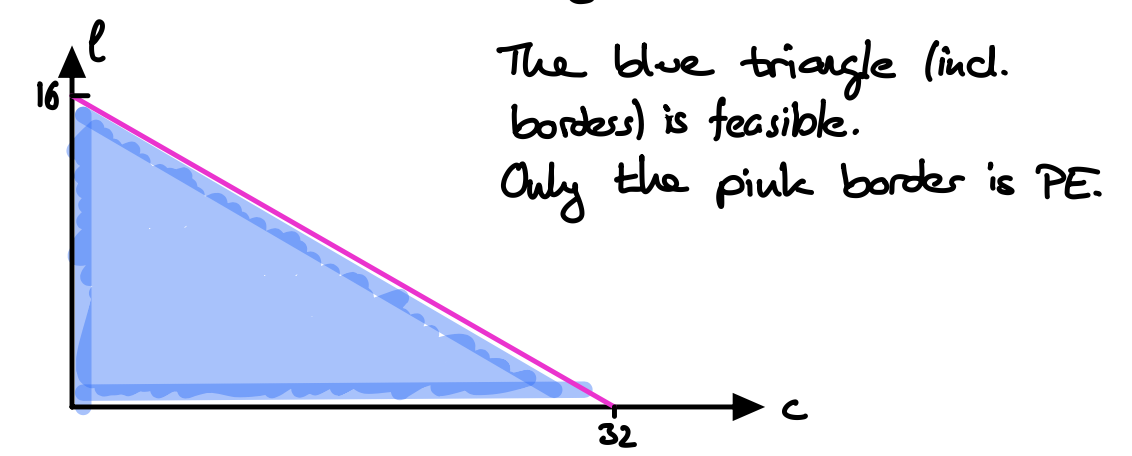
\includegraphics[width=.75\textwidth]{images/2020_21_1.png}
\end{figure}
}
{\item 
\underline{consumer:}

\begin{align*}
    \max _{c, l} \ln (c)+\ln (l) \\
    \text { st. } p c+w l=16 w
\end{align*}

FOCs:

\begin{align*}
    & \frac{1}{c}-\lambda p=0 \\
    & \frac{1}{c}-\lambda w=0 \\
    &\rightarrow c=\frac{w}{p} l
\end{align*}

\underline{Firm:}

\begin{align*}
    \max P A L-w L
\end{align*}

$$
L=\left\{\begin{array}{lll}
\infty & \text { if } & A \geq w / p \\
\mathbb{R}^{+} & \text {if } & A \geq w / p \\
0 & \text { if } & A<w / p
\end{array}\right.
$$

\underline{Markets:}

\begin{align*}
    L=16-l \longrightarrow w / p=A=2
\end{align*}

$$
\begin{aligned}
& \left\lvert\, \begin{array}{l}
c=y=A L=A(16-l)=32-2 l \\
c=\frac{w}{p}l=A l=2 l
\end{array}\right\rvert\, \\
& \longrightarrow l=8 ; L=8 ; c=y=16
\end{aligned}
$$

\underline{Competitive Equilibrium:}

\begin{align*}
    w / p=2 \\
    y=16 \\
    L=8
\end{align*}

Since $c=32-2 l$ holds, the $C E$ is $P E$.
}
{\item 
(1) $\frac{w}{p}$ will increase, as $\frac{w}{p}=A^{\prime}$. Else, we'd have $\frac{w}{p}<A^{\prime}$ and the firm would demand infinite labour. This excess demand cannot exist in a CE.

(2) $y$ must increase. More productive firm increases its output.

(3) $L$ remains the same. The firm produces more at a lower price and the consumer consumes more, working the same for a higher relative wage. She could work more and consume more but since $MRS =c / l$, this is not what happens.

The utility increases as $l=8$ as before but $c$ increases as $y$ increases.
}
\end{enumerate}
}
{
\subsubsection*{Exercise 2}
Yes. If one of the consumers has non-convex preferences, we con find prices at PE allocations that are not CE:

\begin{figure}[!htp]
    \centering
    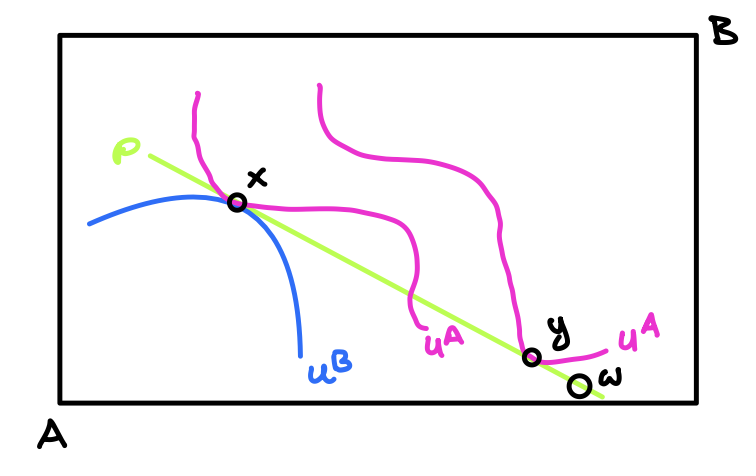
\includegraphics[width=.75\textwidth]{images/2020_21_2.png}
\end{figure}

Although $x$ is PE, A could be better off at these prices. Therefore $x$ is not a CE.
}
{
\subsubsection*{Exercise 3}

\begin{align*}
    w^{A}=(4,8) \quad ; \quad w^{B}=(2,1)
\end{align*}

\begin{enumerate}[label=(\alph*)]
{\item 
$$
MRS^{A}=\frac{1 / 2 x_{2}^{A}}{1 / 2 x_{1}^{A}} \stackrel{!}{=} M R S^{B}=1 \rightarrow x_{2}^{A}=x_{1}^{A}
$$

All PE-allocation are in blue.

\begin{figure}[!htp]
    \centering
    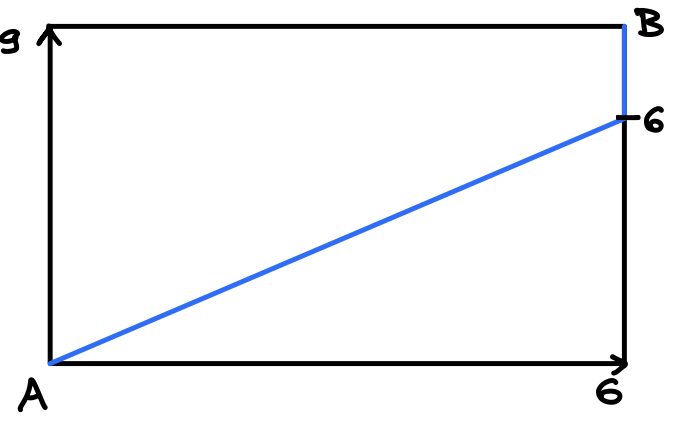
\includegraphics[width=.75\textwidth]{images/2020_21_3.png}
\end{figure}
}
{\item 
\underline{consumer A:}

\begin{align*}
    & \max_{x_{1}^{A}, x_{2}^{A}} 1 / 2\left(\ln \left(x_{1}^{A}\right)+\ln \left(x_{2}^{A}\right)\right) \\
    \text { s.t. } & q_{1} \theta_{1}^{A}+q_{2} \theta_{2}^{A}=0 \\
    & x_{1}^{A}=w_{1}^{A}+\theta_{1}^{A} \\
    & x_{2}^{A}=w_{2}^{A}+\theta_{2}^{A}
\end{align*}

\begin{align*}
    \Longleftrightarrow \quad \max _{x_{1}^{A} , x_{2}^{A}} 1 / 2\left(\ln \left(x_{1}^{A}\right)+\ln \left(x_{2}^{A}\right)\right) \\
    \text{s.t. } q_{1}\left(x_{1}^{A}-w_{1}^{A}\right)+q_{2}\left(x_{2}^{A}-w_{2}^{A}\right)=0
\end{align*}

FOCs:

\begin{align*}
    \left[x_{1}^{A}\right]: \frac{1}{2 x_{1}^{A}}-\lambda q_{1} & =0 \\
    {\left[x_{2}^{A}\right]: \frac{1}{2 x_{2}^{A}}-\lambda q_{2} } & =0 \\
    \rightarrow \frac{q_{1}}{q_{2}} &=\frac{x_{2}^{A}}{x_{1}^{A}} \tag{I}
\end{align*}

\underline{consumer B:}

\begin{align*}
    \max_{x_{1}^{\beta} x_{2}^{\beta}} 1 / 2\left(x_{1}^{\beta}+x_{2}^{\beta}\right) \\
    \text { s.t. } q_{1}\left(x_{1}^{B}-w_{1}^{D}\right)+q_{2}\left(x_{2}^{8}-w_{1}^{B}\right)=0 
\end{align*}

FOCs:


\begin{align*}
    \left[x_{1}^{B}\right]: 1 / 2+\lambda q_{1}=0 \\
    \left[x_{2}^{B}\right]: 1 / 2+\lambda q_{2}=0 \\
    \rightarrow \frac{q_{1}}{q_{2}}=1 \tag{II}
\end{align*}

Plug (II) into (I):

\begin{align*}
    x_{2}^{A}=x_{1}^{A} \tag{III}
\end{align*}

Use (II) and (III) in BC for $A$ :

$$
x_{1}^{A}=x_{2}^{A}=\frac{w_{1}^{A}+w_{2}^{A}}{2}=6
$$

\underline{markets:}

$$
\begin{aligned}
& x_{1}^{A}+x_{1}^{B}=w_{1}^{A}+w_{1}^{B}=6 \\
& \longrightarrow x_{1}^{B}=0 \\
& x_{2}^{A}+x_{2}^{B}=w_{2}^{A}+w_{2}^{B}=9 \\
& \longrightarrow x_{2}^{B}=3
\end{aligned}
$$

\underline{Competitive Equilibrium:}

$$
\begin{aligned}
\left(x_{1}^{A}, x_{2}^{A}\right) & =(6,6) \\
\left(x_{1}^{B}, x_{2}^{B}\right) & =(0,3) \\
\frac{q_{1}}{q_{2}} & =1
\end{aligned}
$$
}
{\item 

PE:

\begin{align*}
    M R S^{A}=x_{2}^{A} / x_{1}^{A} \stackrel{!}{=} M R S^{B}=1 / 3 \\
    \longrightarrow x_{2}^{A}=\frac{1}{3} x_{1}^{A}
\end{align*}

The new set of PE-allocations is indicated in pink.

\begin{figure}[!htp]
    \centering
    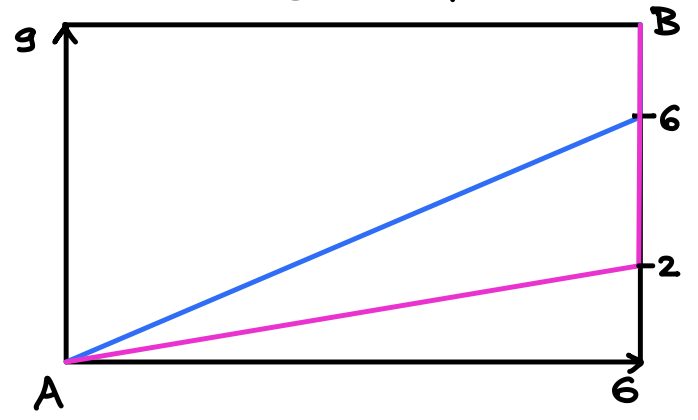
\includegraphics[width=.75\textwidth]{images/2020_21_4.png}
\end{figure}

Now $\frac{q_{1}}{q_{2}}=\frac{1}{3}$. Reason being that the prices of the Arrow-securities reflect the state-probabilities of the risk-neutral agent as she will take on the entire risk in equilibrium.
}
\end{enumerate}
}
}